\documentclass[
	parskip=half,
	a4paper,
]{scrarticle}

\usepackage{xcolor}
\definecolor{seeblau}{HTML}{00A9E0}
\definecolor{seegrau}{HTML}{9AA0A7}

\definecolor{seeblau1}{HTML}{CCEEF9}
\definecolor{seeblau2}{HTML}{A6E1F4}
\definecolor{seeblau3}{HTML}{59C7EB}
\definecolor{seeblau4}{HTML}{00A9E0}
\definecolor{seeblau5}{HTML}{008ECE}


\usepackage{graphicx}
\usepackage{amsmath}
\usepackage{subcaption}
\usepackage{wrapfig}
\usepackage[english]{babel}
\usepackage{blindtext}
\usepackage{microtype}
\usepackage{siunitx}
\usepackage[utf8]{inputenc}
\usepackage{csquotes}
\usepackage{nicefrac}
\usepackage[T1]{fontenc}
\usepackage{amsfonts}
\usepackage{amssymb}
\usepackage{tikz}
\usepackage{parskip}

\usepackage{libertinus, libertinust1math}
\usepackage[sfdefault]{biolinum}
\usepackage{roboto}

\setkomafont{disposition}{\normalfont\sffamily}

% set margins
\usepackage{geometry}
\geometry{
	a4paper,
	left=2.5cm,
	right=2.5cm,
	top=2.5cm,
	bottom=2.5cm
}

% caption
\usepackage{caption}
\captionsetup{
	% font={sf},
	labelfont={sf, bf, color=seeblau},
	labelsep=quad,
	labelformat=simple,
}

% links
\usepackage{hyperref}
\hypersetup{
	colorlinks=true,
	linkcolor=seeblau,
	citecolor=seeblau,
	urlcolor=seeblau,
	% hidelinks=true
}

% bibliography
\usepackage[
	style=numeric-comp, % comp = compressed 4,5,6,7 -> 4-7
	sorting=none,		% Sort by appearance
	% autocite = superscript,
	% backref=true,
	hyperref=true,
	url=true,
	maxbibnames=100
]{biblatex}

\usepackage{float}
% \floatplacement{figure}{h}
% \floatplacement{table}{H}

% loosen float placement rules
\renewcommand{\topfraction}{0.8}
\renewcommand{\bottomfraction}{.8}
\renewcommand{\textfraction}{0.1}
\renewcommand{\floatpagefraction}{.9}
% make floats less likely to be placed on a separate page
\setcounter{totalnumber}{9}
\setcounter{topnumber}{9}
\setcounter{bottomnumber}{9}

% decrease space between floats and text
\setlength{\textfloatsep}{0.25cm}
\setlength{\floatsep}{0.25cm}

% decrease space after disposition
\RedeclareSectionCommands[
	afterskip=1px
]{section, subsection, subsubsection}

\usepackage{adjustbox}

\usepackage{datetime}
\newdateformat{dotdate}{
	\twodigit{\THEDAY}.\twodigit{\THEMONTH}.\THEYEAR
}
\newdateformat{monthyeardate}{%
  \monthname[\THEMONTH] \THEYEAR}


% header and footer
\usepackage[
  markcase=noupper
]{scrlayer-scrpage}% activates pagestyle scrheadings automatically
\clearpairofpagestyles
\setkomafont{pageheadfoot}{\normalfont\sffamily}
\setkomafont{pagenumber}{\normalfont\sffamily}
% \chead*{\color{seegrau} Draft \dotdate\today}
\ofoot*{\pagemark}
\ohead*{\rightmark}


\usepackage{ifthen}
\newcommand{\markieren}[4]{
	\ifthenelse{\equal{#1}{}}{}{\adjustbox{padding=3pt, bgcolor=seeblau1, margin=-1pt}{\strut{\sffamily\robotoMedium{#1}}}\\}
  \ifthenelse{\equal{#2}{}}{}{\adjustbox{padding=3pt, bgcolor=seeblau2, margin=-1pt}{\strut{\sffamily\robotoMedium{#2}}}\\}
	\ifthenelse{\equal{#3}{}}{}{\adjustbox{padding=3pt, bgcolor=seeblau3, margin=-1pt}{\strut{\sffamily\robotoMedium{#3}}}\\}
	\ifthenelse{\equal{#4}{}}{}{\adjustbox{padding=3pt, bgcolor=seeblau4, margin=-1pt}{\strut{\sffamily\robotoMedium{#4}}}}
}

\addbibresource{../literature.bib}
\begin{document}

\title{Procedures for Hot Electron Measurements}
\author{Leon Oleschko}
\date{\dotdate\today}

\begin{titlepage}
    \sffamily
    \vspace*{3cm}
    {
        \fontsize{32}{32}
        \markieren{}{Hot Electron}{Thermal Emission}{Spectroscopy}
    }
    \vspace{.25cm}\\
    {
        \Large
        Leon Oleschko\\
        Supervised by Peter Baum
        \vspace{.05cm}\\
        \dotdate\today\\
        % \vspace{.25cm}\\
        % \normalsize
        Universität Konstanz
    }
    \vfill
    {
        \normalfont\normalsize

    }
    \vfill
    \begin{flushright}
        Available at \url{www.github.com/leoole100/projekt-praktikum}.
    \end{flushright}
\end{titlepage}

% {
% 	\sffamily
% 	\hypersetup{hidelinks}
% 	\tableofcontents
% }

\clearpage


\addcontentsline{toc}{section}{Introduction}
\section*{Introduction}

\section{Experimental Setup}
The experimental setup, originally designed by Leon Roob \autocite{roob_thermal_2025}, enables measurement of thermal radiation from ultrafast hot electrons. It follows the principles of typical ultrafast photoemission spectroscopy \autocite{lui_ultrafast_2010}, combining femtosecond laser excitation with precise collection optics and spectral detection. Thermal emission from the sample is collected by parabolic mirrors and analysed using a monochromator equipped with a blazed diffraction grating, with detection performed by an EMCCD camera. The following sections describe the collection optics, the monochromator, and the detector in more detail.


\subsection{Collection}
Thermal radiation emitted by the excited hot electrons is collected using two off-axis parabolic aluminium mirrors. The first parabolic mirror (PM1), with a diameter of \SI{50.8}{\milli\meter} and a focal length of \SI{50.8}{\milli\meter}, collimates the emitted light from the sample. A second parabolic mirror (PM2), structurally identical but with a focal length of \SI{101.6}{\milli\meter}, focuses the collimated radiation into an optical fibre leading to the monochromator. This geometry ensures efficient light collection over a broad solid angle, which is critical given the low photon flux characteristic of ultrafast thermal emission measurements.

To suppress residual laser fundamental radiation, two Schott KG3 infrared filters are placed between PM2 and the fibre input. These filters exhibit high transmittance between \SI{360}{\nano\meter} and \SI{590}{\nano\meter} but attenuate light outside this range to less than \SI{0.1}{\percent}. Both filters are tilted to prevent back reflections into the optical path, though this tilt reduces their maximum transmission to around \SI{20}{\percent} per filter for visible wavelengths. Transmission losses from filters and mirror coatings must be accounted for during system calibration to accurately reconstruct the emission spectrum.

\subsection{Monochromator}
The spectrally resolved analysis of the collected thermal radiation is performed using an Acton SpectraPro 300i monochromator. This instrument employs a ruled diffraction grating with 150 grooves per millimetre and a blaze wavelength of 500 nm. The blazing optimises the grating's diffraction efficiency for visible wavelengths near the blaze wavelength, while efficiency drops off at shorter or longer wavelengths. This wavelength-dependent efficiency curve is a critical factor influencing the measured spectra and must be corrected during calibration procedures to achieve accurate spectral intensity measurements.

The monochromator allows tuning of the central wavelength and control of the spectral bandwidth through adjustable entrance and exit slits. The selection of slit widths is a trade-off between spectral resolution and photon throughput, which is particularly important for weak signals from ultrafast thermal emission.

\subsection{Detector}
Spectrally dispersed thermal radiation is detected using an Andor iXonEM+ CCD camera. Although this camera features an electron multiplication (EM) register capable of amplifying low-light signals, in this setup the EM feature is disabled. Initial tests showed that electron multiplication introduced excess noise, ultimately reducing the signal-to-noise ratio (SNR). Instead, measurements are performed in conventional CCD mode, which provides better overall sensitivity for the photon flux levels encountered in thermal emission experiments.

The detector's quantum efficiency peaks in the visible spectral range but drops significantly below approximately 480 nm, as specified in the manufacturer's datasheet \autocite{andor_ixonem_nodate}. This wavelength-dependent response must be considered when analysing measured spectra, and corrections may be required to reconstruct the true emission profile. In addition, variations in quantum efficiency between individual cameras can introduce systematic errors, highlighting the need for in-situ calibration to ensure quantitative accuracy.


\section{Noise Sources and SNR Optimisation}

Measurements of thermal radiation from ultrafast hot electrons require detection of extremely weak optical signals. The total noise in these measurements arises from several independent sources, each contributing to the uncertainty in the recorded pixel signal. The combined noise can be approximated as

\begin{equation}
    \sigma_{\text{total}} = \sqrt{\sigma_{\text{bias}}^2 + \sigma_{\text{read}}^2 + \sigma_{\text{dark}}^2 + \sigma_{\text{shot}}^2 + \sigma_{\text{CIC}}^2}.
\end{equation}

\paragraph{Bias Noise}

Bias noise refers to small fluctuations in the electronic offset added to all pixel values, typically constant and independent of exposure time. For scientific CCD cameras, this noise is on the order of $1$--$2~e^{-}$~RMS.

\paragraph{Readout Noise}

Readout noise arises during charge-to-voltage conversion and digitisation in the detector electronics. Without electron multiplication (EM) gain, this noise typically amounts to $2$--$5~e^{-}$~RMS. An important consideration is that readout noise scales \emph{per readout bin}. This means that summing multiple pixels via hardware binning before digitisation can significantly reduce the overall noise, because only a single readout noise contribution is added for the binned superpixel rather than for each individual pixel. Hardware binning is therefore advisable wherever spatial or spectral resolution permits.

In EM mode, the effective readout noise is reduced because the signal is amplified before readout, but the amplification process introduces additional noise contributions such as clock-induced charge.

\paragraph{Thermal Noise (Dark Current Noise)}

Thermal noise, also known as dark current noise, originates from thermally generated electrons that accumulate during the exposure time. It follows Poisson statistics and is calculated as

\begin{equation}
    \sigma_{\text{dark}} = \sqrt{I_{\text{dark}} \cdot t_{\text{exp}}},
\end{equation}

where $I_{\text{dark}}$ is the dark current in electrons per second per pixel, and $t_{\text{exp}}$ is the exposure time in seconds.

The dark current itself depends exponentially on the sensor temperature according to

\begin{equation}
    I_{\text{dark}}(T) = I_0 \cdot \exp\left(-\frac{E_{\text{gap}}}{k T}\right),
\end{equation}

where $I_0$ is a pre-exponential factor determined by the device, $E_{\text{gap}}$ is the effective activation energy (typically around $0.6$--$0.7$~eV for silicon), $k$ is the Boltzmann constant, and $T$ is the absolute temperature in Kelvin. This relationship highlights the importance of cooling the sensor to achieve low-noise measurements.

\paragraph{Shot Noise}

Shot noise reflects the statistical nature of photon arrival and is given by

\begin{equation}
    \sigma_{\text{shot}} = \sqrt{S},
\end{equation}

where $S$ is the signal in electrons. Shot noise is fundamentally unavoidable but decreases in relative terms as the signal increases, since the signal-to-shot-noise ratio improves proportionally to $\sqrt{S}$.

\paragraph{Clock-Induced Charge (CIC)}

An additional noise source relevant to EM gain mode is clock-induced charge (CIC). CIC arises from spurious electrons generated during rapid voltage changes as pixel charges are shifted through the EM register. This noise becomes significant in low-light measurements, particularly at high EM gain. It can be approximated as

\begin{equation}
    \sigma_{\text{CIC}} = \sqrt{N_{\text{CIC}} \times \text{EM}_{\text{gain}}^2},
\end{equation}

where $N_{\text{CIC}}$ denotes the average number of CIC electrons per pixel per frame, and $\text{EM}_{\text{gain}}$ is the electron multiplication gain factor. High EM gain amplifies both the signal and CIC, potentially reducing the overall signal-to-noise ratio (SNR).

\paragraph{Implications for SNR Optimisation}

From a practical perspective, these considerations imply that lower EM gain and longer exposure times are generally beneficial for achieving a higher SNR. Longer exposures increase the total collected signal, improving the shot noise-limited SNR, while also reducing the relative contribution of frame-based noises like CIC. However, longer exposure times also increase dark noise, which must be mitigated through sufficient sensor cooling.

In the measurements performed for this work, the electron multiplication feature of the Andor iXonEM+ camera was disabled. Tests showed that EM gain introduced significant additional noise, including CIC, which degraded the overall SNR. Instead, data acquisition was performed in conventional CCD mode, using longer exposure times, sensor cooling, and hardware binning where possible, to optimise sensitivity while maintaining acceptable noise levels.

\begin{figure}
    \centering
    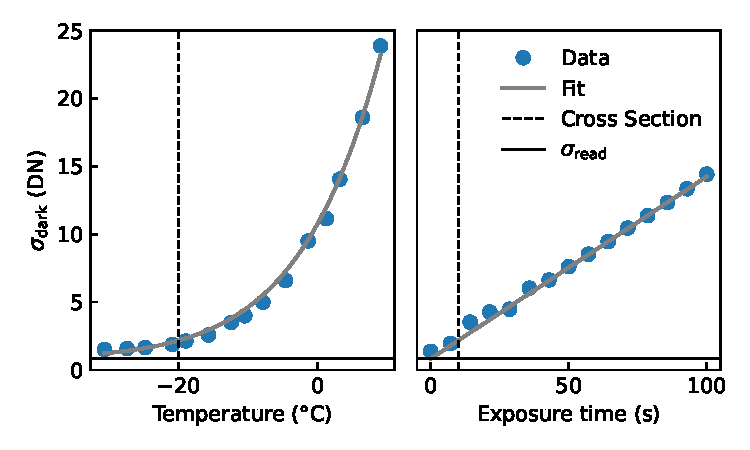
\includegraphics{../analysis/figures/dark_noise.pdf}
    \caption{Dark noise over Temperature and Exposure Time. With modeled $E_\text{gap} = \SI{0.613(6)}{eV}$ and a constant Readout noise of $\sigma_{\text{read}} = \SI{0.88(12)}{e^-}$.}
\end{figure}


\section{Flatness and Efficiency}

\addcontentsline{toc}{section}{Concolusion}
\section*{Conclusion}

\clearpage
\printbibliography

\end{document}